% !TeX program = xelatex
\documentclass[10pt]{beamer}

\usetheme{metropolis}

\usepackage{pgfplots}
\usepgfplotslibrary{fillbetween}
\usepackage{pgfopts}
\usepackage{amsmath}
\usepackage{structuralanalysis}
\usepackage{tikz}
\usepackage{tikz-3dplot}
\usepackage{chngcntr}
\usepackage{wasysym}
\usepackage{mathtools}
\usepackage{alphalph}
\usepackage{xcolor}
\usepackage[showdow=false, en-US]{datetime2}

\newcommand{\highlight}[1]{%
	\colorbox{red!50}{$\displaystyle#1$}}

\setcounter{lecture}{10}
\counterwithin{equation}{lecture}
\makeatletter
\def\user@resume{resume}
\def\user@intermezzo{intermezzo}
%
\newcounter{previousequation}
\newcounter{lastsubequation}
\newcounter{savedparentequation}
\setcounter{savedparentequation}{1}
% 
\renewenvironment{subequations}[1][]{%
	\def\user@decides{#1}%
	\setcounter{previousequation}{\value{equation}}%
	\ifx\user@decides\user@resume 
	\setcounter{equation}{\value{savedparentequation}}%
	\else  
	\ifx\user@decides\user@intermezzo
	\refstepcounter{equation}%
	\else
	\setcounter{lastsubequation}{0}%
	\refstepcounter{equation}%
	\fi\fi
	\protected@edef\theHparentequation{%
		\@ifundefined {theHequation}\theequation \theHequation}%
	\protected@edef\theparentequation{\theequation}%
	\setcounter{parentequation}{\value{equation}}%
	\ifx\user@decides\user@resume 
	\setcounter{equation}{\value{lastsubequation}}%
	\else
	\setcounter{equation}{0}%
	\fi
	\def\theequation  {\theparentequation  \alph{equation}}%
	\def\theHequation {\theHparentequation \alph{equation}}%
	\ignorespaces
}{%
%  \arabic{equation};\arabic{savedparentequation};\arabic{lastsubequation}
\ifx\user@decides\user@resume
\setcounter{lastsubequation}{\value{equation}}%
\setcounter{equation}{\value{previousequation}}%
\else
\ifx\user@decides\user@intermezzo
\setcounter{equation}{\value{parentequation}}%
\else
\setcounter{lastsubequation}{\value{equation}}%
\setcounter{savedparentequation}{\value{parentequation}}%
\setcounter{equation}{\value{parentequation}}%
\fi\fi
%  \arabic{equation};\arabic{savedparentequation};\arabic{lastsubequation}
\ignorespacesafterend
}
\makeatother
\title{AE 737 - Mechanics of Damage Tolerance}
\subtitle{Lecture \arabic{lecture}}
\date{Last Updated: \today\ at \DTMcurrenttime}
\author{Dr. Nicholas Smith}
\institute{Wichita State University, Department of Aerospace Engineering}
% \titlegraphic{\hfill\includegraphics[height=1.5cm]{logo/logo}}

\begin{document}

\maketitle
\begin{frame}{schedule}
	\begin{itemize}
		\item 23 Feb - Residual Strength, Multiple Site Damage
		\item 25 Feb - Multiple Site Damage, Mixed-mode Fracture, Homework 4 Due, Homework 5 Assigned
		\item 1 Mar - Section 1 Review, Homework 5 Due
		\item 3 Mar - Section 1 Review, Homework 5 return
		\item 8 Mar - Exam 1
		\item 10 Mar - Exam return, Final Project discussion
	\end{itemize}
\end{frame}

\begin{frame}
  \frametitle{outline}
  \setbeamertemplate{section in toc}[sections numbered]
  \tableofcontents[hideallsubsections]
\end{frame}

\section{residual strength review}

%5-10 minutes
\begin{frame}{residual strength review}
	\begin{itemize}
		\item Group 1 - Sketch a residual strength curve for a single material (include fracture and net-section yield)
		\item Group 2 - Sketch and describe the difference in residual strength between stiff/brittle materials and ductile/tough materials
		\item Group 3 - Find the proof load needed to ensure no center-cracks less than 0.01" are present in a material with $K_C = 120 \text{ ksi}\sqrt{\text{in.}}$
		\item Group 4 - Sketch the Fedderson approach to residual strength. How is this different from the traditional approach? Why is it beneficial?
	\end{itemize}
\end{frame}

\section{stiffeners}

\begin{frame}{stiffened panels}
	\begin{itemize}[<+->]
		\item In aircraft the skin/stringer system provides many benefits (resistance to buckling)
		\item Stringers also act as stiffeners to resist crack propagation in the skin
		\item Panels in these configurations are generally very wide relative to expected crack dimensions
		\item Cracks are generally modeled either as centered between stiffeners or centered under a stiffener
		\item We need to consider the residual strength of the panel, the stiffener, and the rivets
	\end{itemize}
\end{frame}

\begin{frame}{centered between stiffeners}
	\begin{figure}[H]
		\centering
		\begin{tikzpicture}
		\begin{scope}[scale=0.25]
		\point{a}{0}{1.5};
		\point{b}{10}{1.5};
		\point{c}{0}{-1.6};
		\point{d}{10}{-1.6};
		\draw (0,3) -- (40,3) -- (40,-3) -- (0,-3) -- (0,3);
		\draw (2,3) -- (3,3) -- (3,-3) -- (2,-3) -- (2,3);
		\draw (14,3) -- (15,3) -- (15,-3) -- (14,-3) -- (14,3);
		\draw (26,3) -- (27,3) -- (27,-3) -- (26,-3) -- (26,3);
		\draw (38,3) -- (39,3) -- (39,-3) -- (38,-3) -- (38,3);
		\draw[<-] (3,-2) -- (7,-2);
		\draw[->] (10,-2) -- (14,-2);
		\draw node at (8.5,-2) {$b$};
		\draw[<->] (3.5,2) -- (3.5,1);
		\draw node at (9,1.5) {$p = $ rivet pitch};
		\lineload{3}{a}{b}[-2][-2];
		\draw node at (20,8) {$\sigma = S$};
		\lineload{3}{c}{d}[2][2];
		\draw node at (20,-8) {$\sigma = S$};
		\draw (16,0) -- (25,0);
		\draw node at (20.5,1) {$2a$};
		\draw (2.5,0) circle (0.15) (2.5,1)circle (0.15) (2.5,2)circle (0.15) (2.5,-2)circle (0.15) (2.5,-1)circle (0.15);
		\draw (14.5,0) circle (0.15) (14.5,1)circle (0.15) (14.5,2)circle (0.15) (14.5,-2)circle (0.15) (14.5,-1)circle (0.15);
		\draw (26.5,0) circle (0.15) (26.5,1)circle (0.15) (26.5,2)circle (0.15) (26.5,-2)circle (0.15) (26.5,-1)circle (0.15);
		\draw (38.5,0) circle (0.15) (38.5,1)circle (0.15) (38.5,2)circle (0.15) (38.5,-2)circle (0.15) (38.5,-1)circle (0.15);
		\end{scope}
		\end{tikzpicture}
	\end{figure}
\end{frame}

\begin{frame}{centered under stiffener}
	\begin{figure}[H]
		\centering
		\begin{tikzpicture}
		\begin{scope}[scale=0.25]
		\point{a}{0}{1.5};
		\point{b}{10}{1.5};
		\point{c}{0}{-1.6};
		\point{d}{10}{-1.6};
		\draw (22,0) -- (31,0);
		\draw node at (29,1) {$a$};
		\draw node at (24,1) {$a$};
		\draw (0,3) -- (40,3) -- (40,-3) -- (0,-3) -- (0,3);
		\draw (2,3) -- (3,3) -- (3,-3) -- (2,-3) -- (2,3);
		\draw (14,3) -- (15,3) -- (15,-3) -- (14,-3) -- (14,3);
		\draw (26,3) -- (27,3) -- (27,-3) -- (26,-3) -- (26,3);
		\draw (38,3) -- (39,3) -- (39,-3) -- (38,-3) -- (38,3);
		\draw[<-] (3,-2) -- (7,-2);
		\draw[->] (10,-2) -- (14,-2);
		\draw node at (8.5,-2) {$b$};
		\draw[<->] (3.5,2) -- (3.5,1);
		\draw node at (9,1.5) {$p = $ rivet pitch};
		\lineload{3}{a}{b}[-2][-2];
		\draw node at (20,8) {$\sigma = S$};
		\lineload{3}{c}{d}[2][2];
		\draw node at (20,-8) {$\sigma = S$};
		\draw (2.5,0) circle (0.15) (2.5,1)circle (0.15) (2.5,2)circle (0.15) (2.5,-2)circle (0.15) (2.5,-1)circle (0.15);
		\draw (14.5,0) circle (0.15) (14.5,1)circle (0.15) (14.5,2)circle (0.15) (14.5,-2)circle (0.15) (14.5,-1)circle (0.15);
		\draw (26.5,0) circle (0.15) (26.5,1)circle (0.15) (26.5,2)circle (0.15) (26.5,-2)circle (0.15) (26.5,-1)circle (0.15);
		\draw (38.5,0) circle (0.15) (38.5,1)circle (0.15) (38.5,2)circle (0.15) (38.5,-2)circle (0.15) (38.5,-1)circle (0.15);
		\end{scope}
		\end{tikzpicture}
	\end{figure}
\end{frame}

\begin{frame}{remote stress in stiffener}
	\begin{itemize}[<+->]
		\item For equilibrium to be satisfied, we know that 
		\begin{equation*}
		\left(\frac{PL}{AE}\right)_{Skin} = \left(\frac{PL}{AE}\right)_{Stiffener}
		\end{equation*}
		\item Since $L$ is the same, we find
		\begin{equation*}
		\frac{S}{E} = \frac{S_S}{E_S}
		\end{equation*}
		\item Where the subscript $_S$ indicates stiffener values, we can express the remote stress in the stiffener as
		\begin{equation}
		\label{eq:stiff}
		S_S = S \frac{E_S}{E}
		\end{equation}
	\end{itemize}
\end{frame}

\begin{frame}{skin}
	\begin{itemize}[<+->]
		\item The critical stress in the skin is determined the same way as it was in the residual strength chapter
		\item The only exception is that the stiffener contributes to $\beta$
		\begin{equation}
		S_C = \frac{K_C}{\sqrt{\pi a} \beta}
		\end{equation}
	\end{itemize}
\end{frame}

\begin{frame}{stiffener}
	\begin{itemize}[<+->]
		\item The maximum stress in a stiffener will be increased near a crack
		\item We represent the ratio of maximum force in stiffener to remote force with the Stiffener Load Factor, $L$
		\begin{subequations}
		\begin{align}
		L &= \frac{\text{max force in stiffener}}{\text{remote force applied to stiffener}}\\
		&= \frac{S_{S,max}A_S}{S_S A_S}\\
		&= \frac{S_{S,max}}{S \frac{E_S}{E}}\\
		L S \frac{E_S}{E} &= S_{S,max}\\
		L S \frac{E_S}{E} &= \sigma_{YS}\\
		S_C &= \frac{\sigma_{YS} E}{L E_S}
		\end{align}
		\end{subequations}
	\end{itemize}
\end{frame}

\begin{frame}{rivet}
	\begin{itemize}[<+->]
		\item We can define a similar rivet load factor to relate maximum stress in the rivet to remote stress in the skin
		\begin{subequations}
			\begin{align}
			L_R &= \frac{\tau_{max} A_R}{S b t}\\
			L_R &= \frac{\tau_{YS} A_R}{S b t}\\
			S_c &= \frac{\tau_{YS} A_R}{L_R b t}
			\end{align}
		\end{subequations}
	\end{itemize}
\end{frame}

\begin{frame}{finite element analysis}
	\begin{itemize}[<+->]
		\item CC Poe found that panels could be related by a parameter he defines as $\mu$
		\begin{equation}
		\mu = \frac{A_S E_S}{A_S E_S + A E}
		\end{equation}
		\item Where $A_S$ is the cross-sectional area of a stiffener, $E_S$ is stiffener modulus
		\item $A$ is the skin cross-sectional area (per stiffener) $A=b t$ and $E$ is the modulus of the skin
		\item pp 167 - 178 give $\beta$, $L$ and $L_R$ for various skin/stiffener configurations
		\item These values were determined using a finite element model
	\end{itemize}
\end{frame}

\begin{frame}{examples}
	\begin{itemize}
		\item quantitative example (p. 179-180)
		\item qualitative notes on behavior (p. 181-182)
	\end{itemize}
\end{frame}
%TODO real plots for qualitative data (pp. 181-182)

\section{severed stiffeners}

\begin{frame}{failure in stiffener}
	\begin{itemize}[<+->]
		\item Sometimes the stiffeners fail before the panel
		\item T. Swift conducted some parametric studies on panels with a severed stiffener
		\item When the crack is short (and near the severed stiffener) the residual strength is lower due to the broken stiffener
		\item As the crack nears the next stiffener, residual strength is very similar to a panel with all stiffeners intact
	\end{itemize}
\end{frame}

\begin{frame}{failure in stiffener}
	\begin{itemize}[<+->]
		\item Swift considers the difference in stress at different points in the stiffener
		\item Instead of one general load factor ($L$), he uses $SCFO$ and $SCFI$
		\item We can find the critical value of remote stress at the outer flange as
		\begin{equation}
		\sigma_C = \frac{\sigma_U}{SCFO}
		\end{equation}
		\item And similarly at the inner flange
		\begin{equation}
		\sigma_C = \frac{\sigma_U}{SCFI}
		\end{equation}
		\item Swift's parametric study did not consider rivet failure
	\end{itemize}
\end{frame}

%TODO real plots for "qualitative" findings (pp. 184, 186-190)
\begin{frame}{stiffener area}
\begin{figure}
\centering
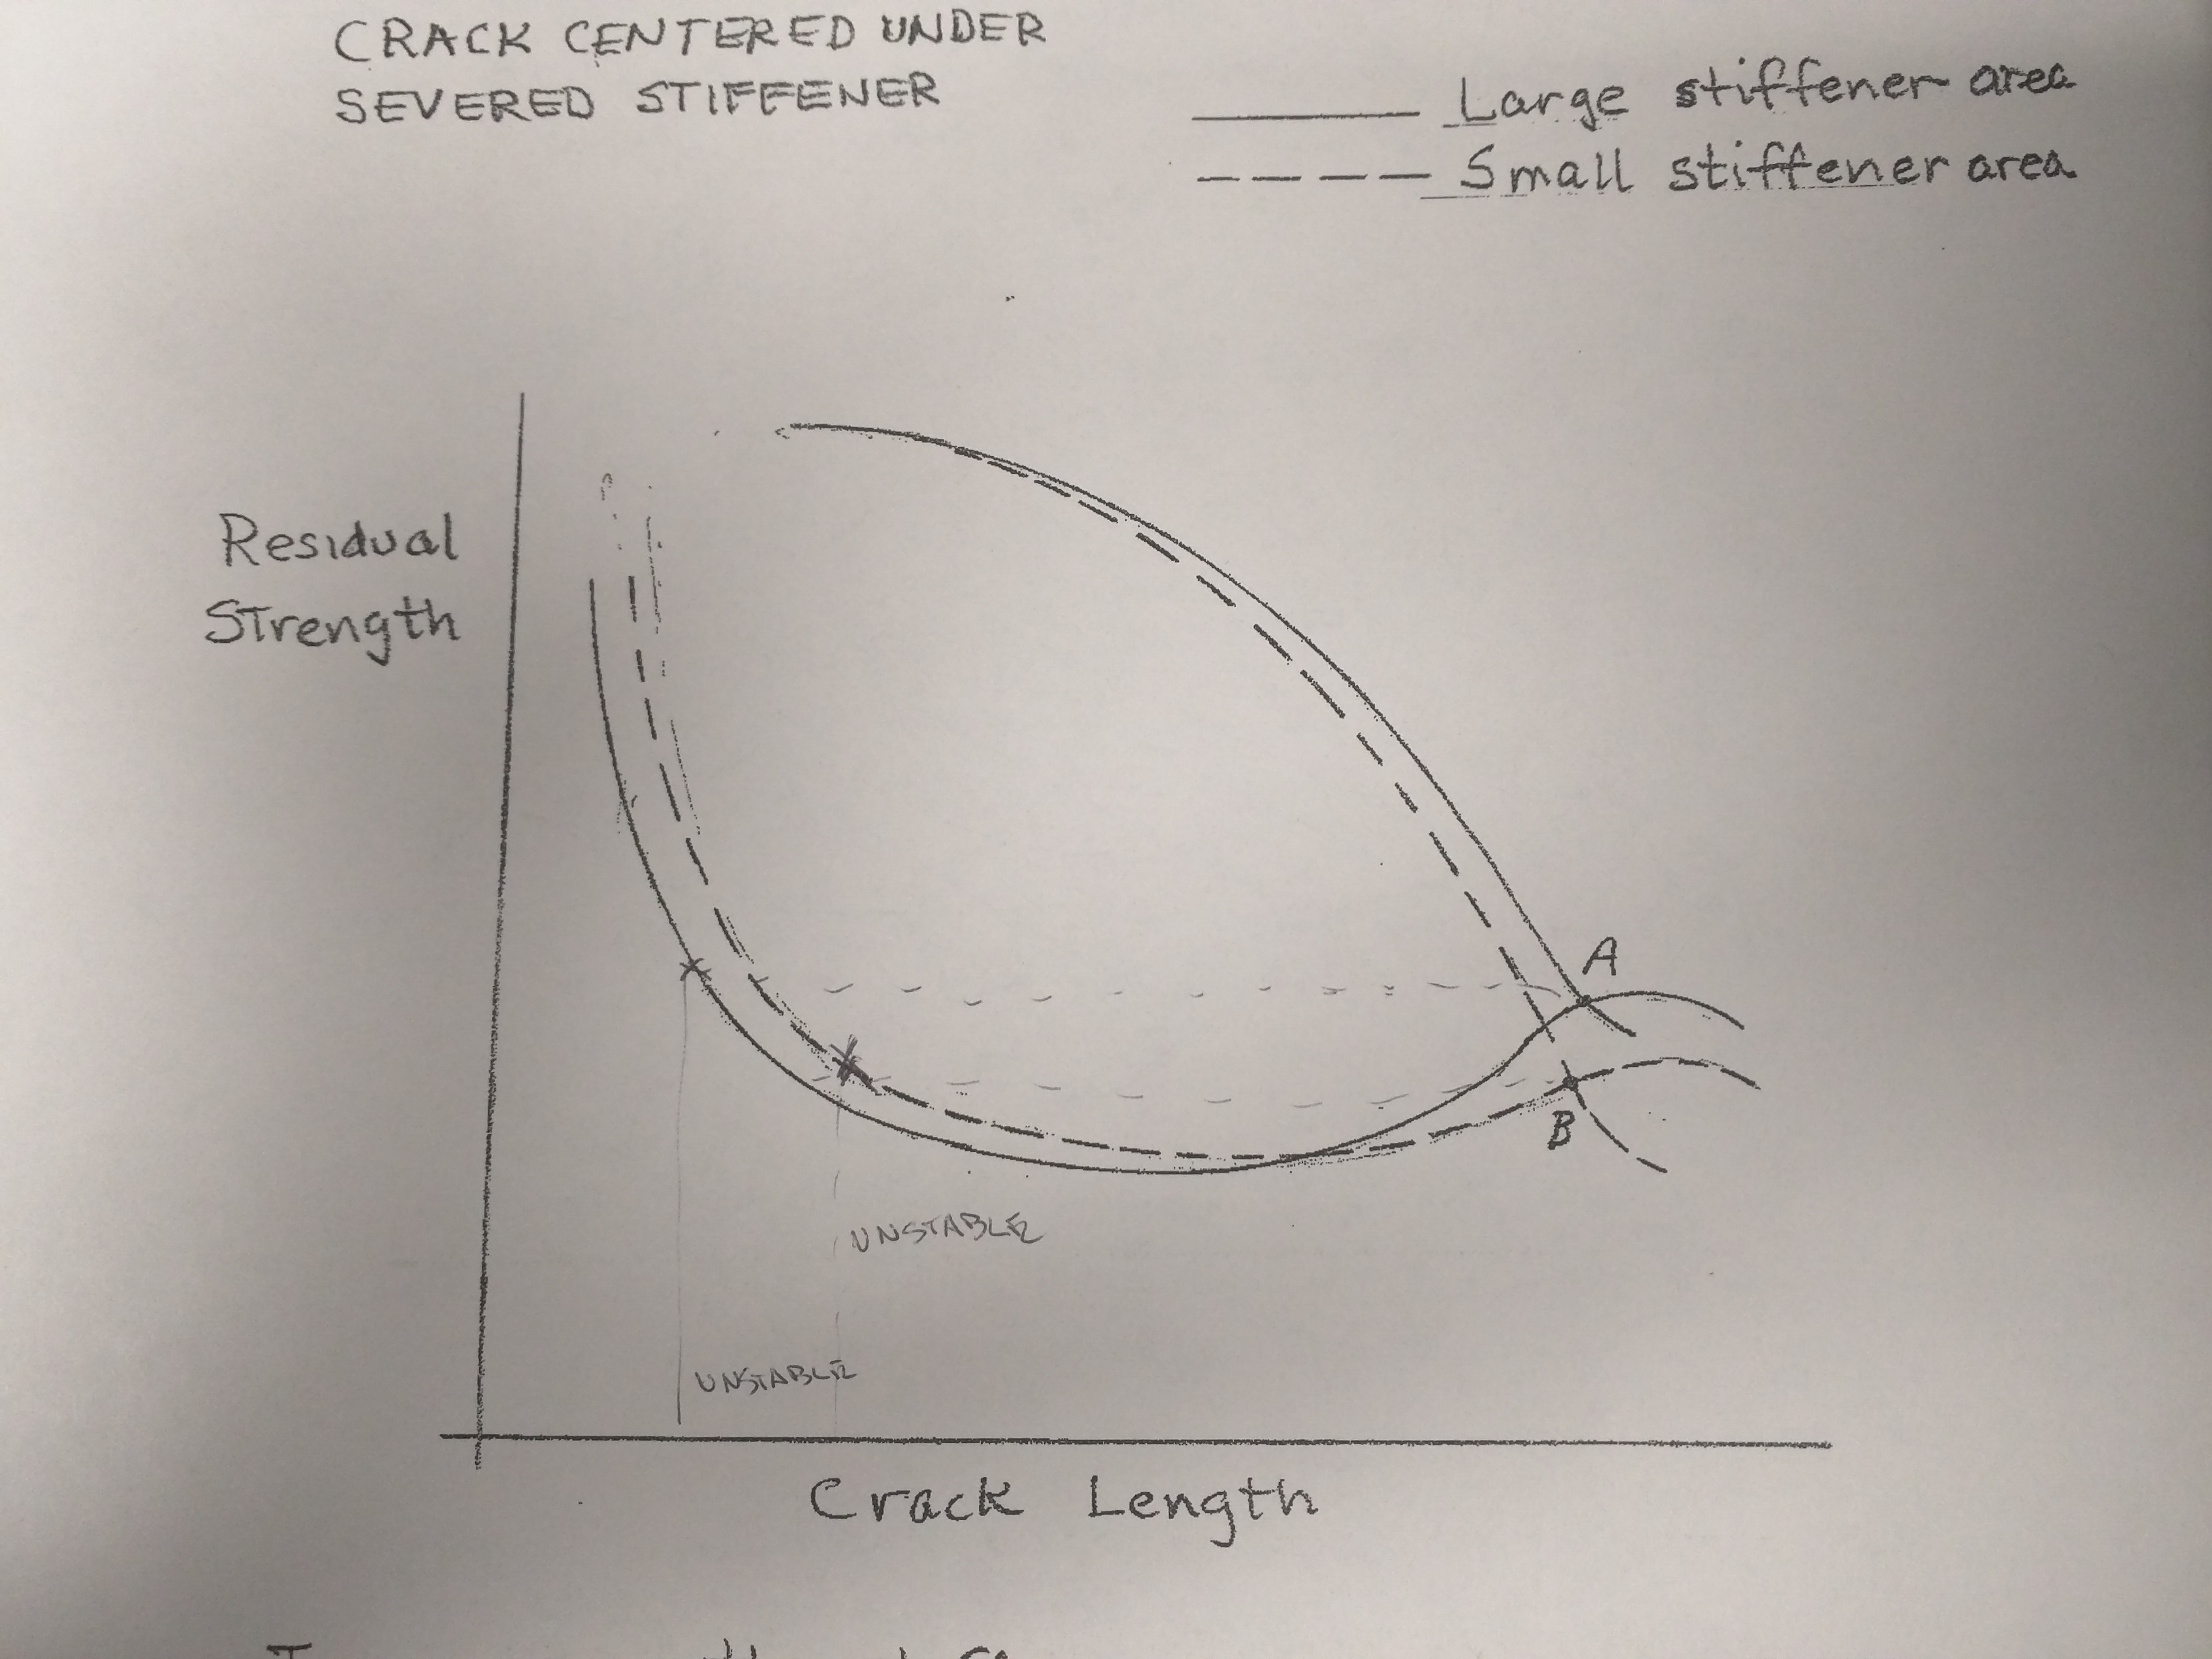
\includegraphics[width=0.7\linewidth]{stiffener_area}
\label{fig:stiffener_area}
\end{figure}
\end{frame}

\begin{frame}{stiffener spacing}
\begin{figure}
\centering
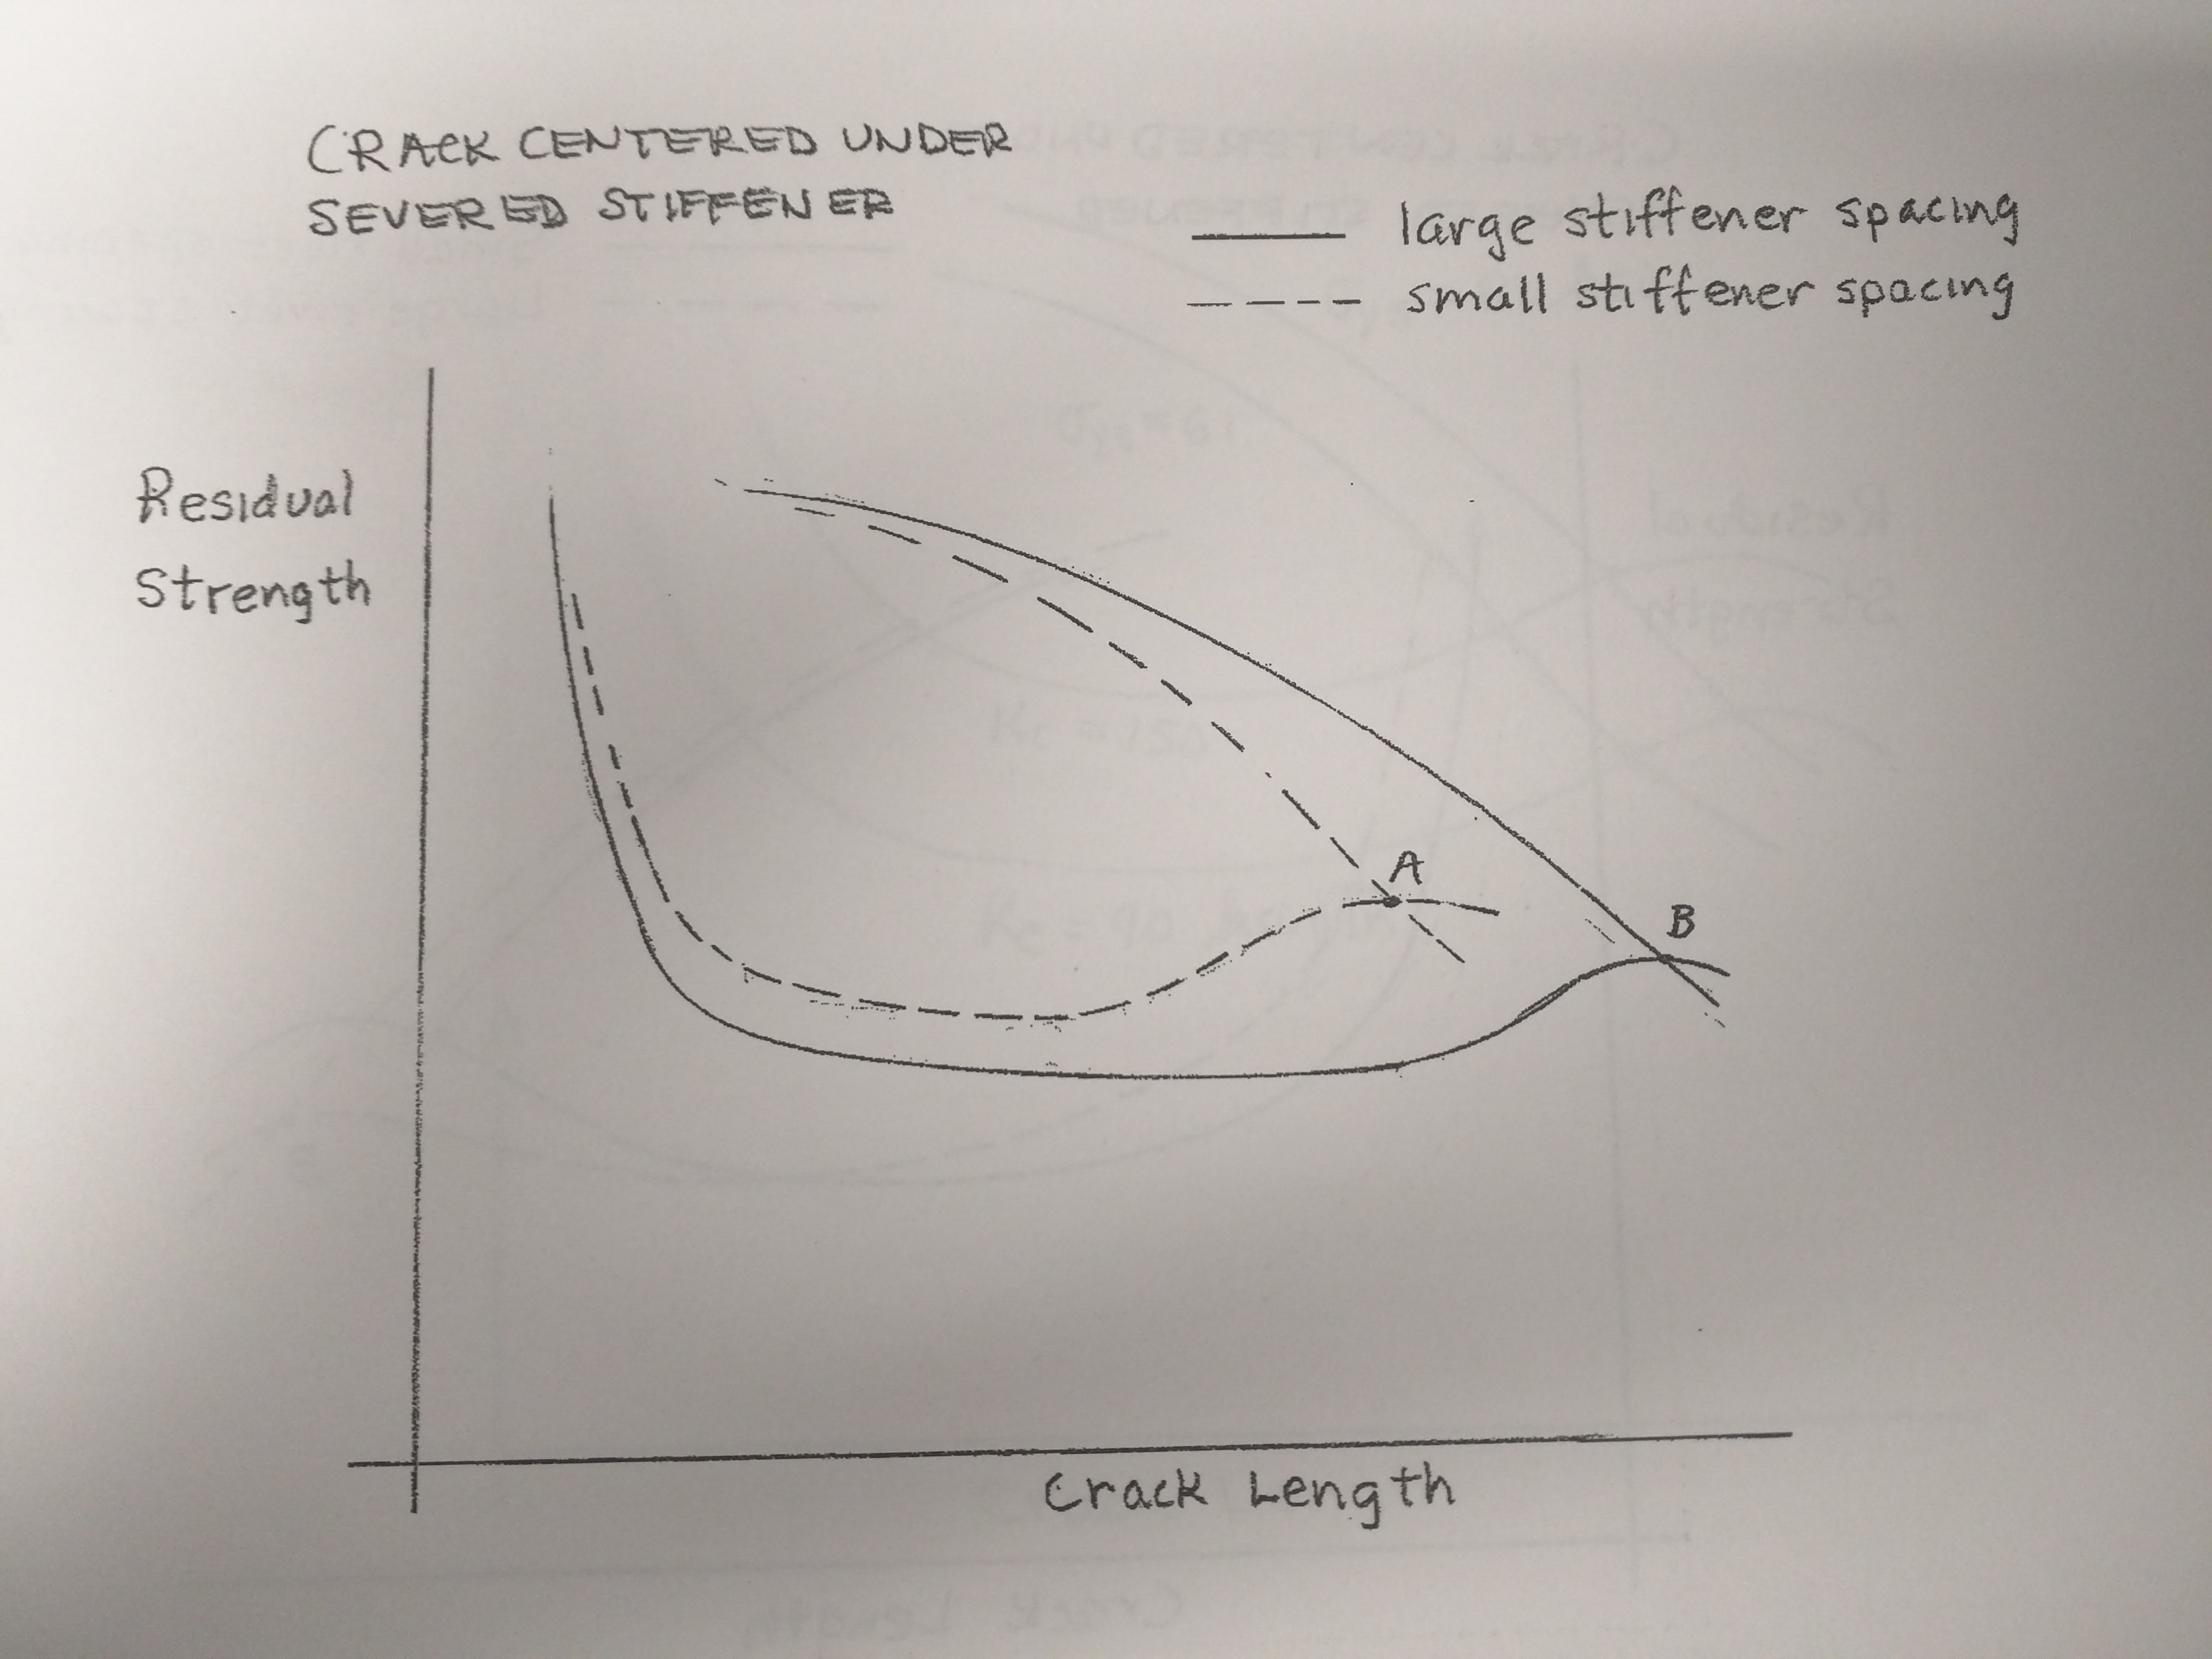
\includegraphics[width=0.7\linewidth]{stiffener_spacing}
\label{fig:stiffener_spacing}
\end{figure}
\end{frame}

\begin{frame}{rivet spacing}
\begin{figure}
\centering
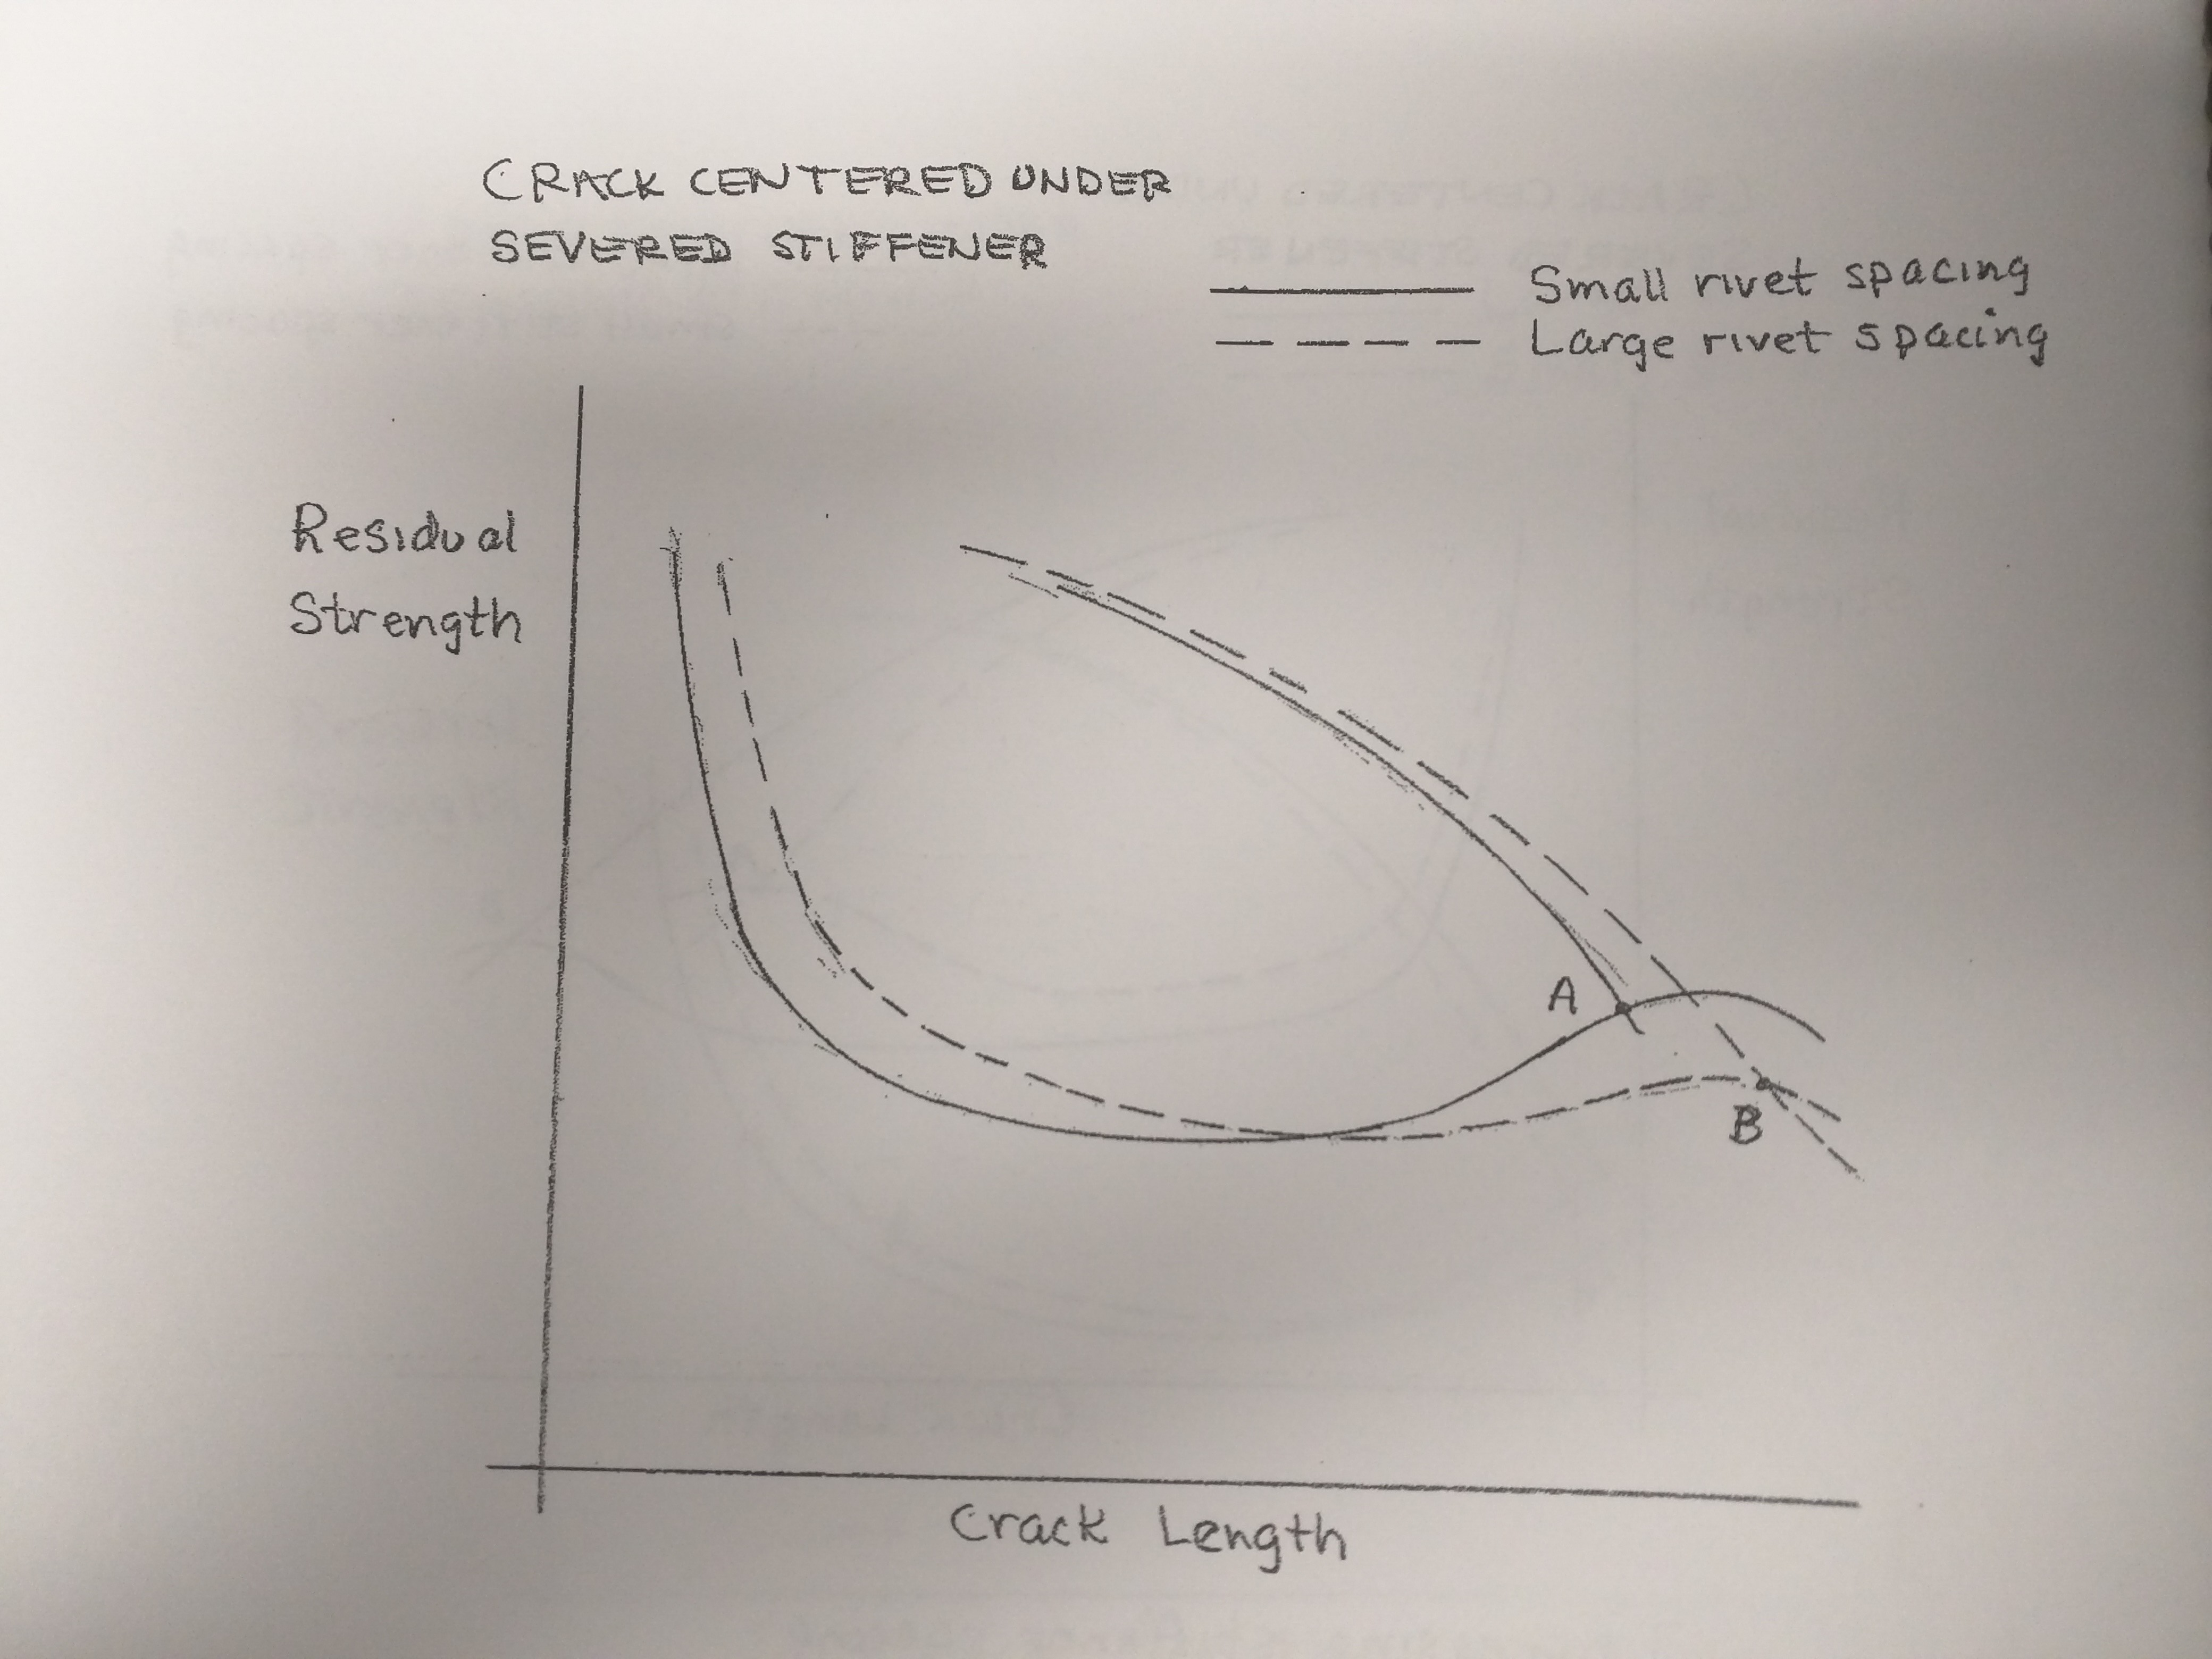
\includegraphics[width=0.7\linewidth]{rivet_spacing}
\label{fig:rivet_spacing}
\end{figure}
\end{frame}

\begin{frame}{strength and toughness increase}
\begin{figure}
\centering
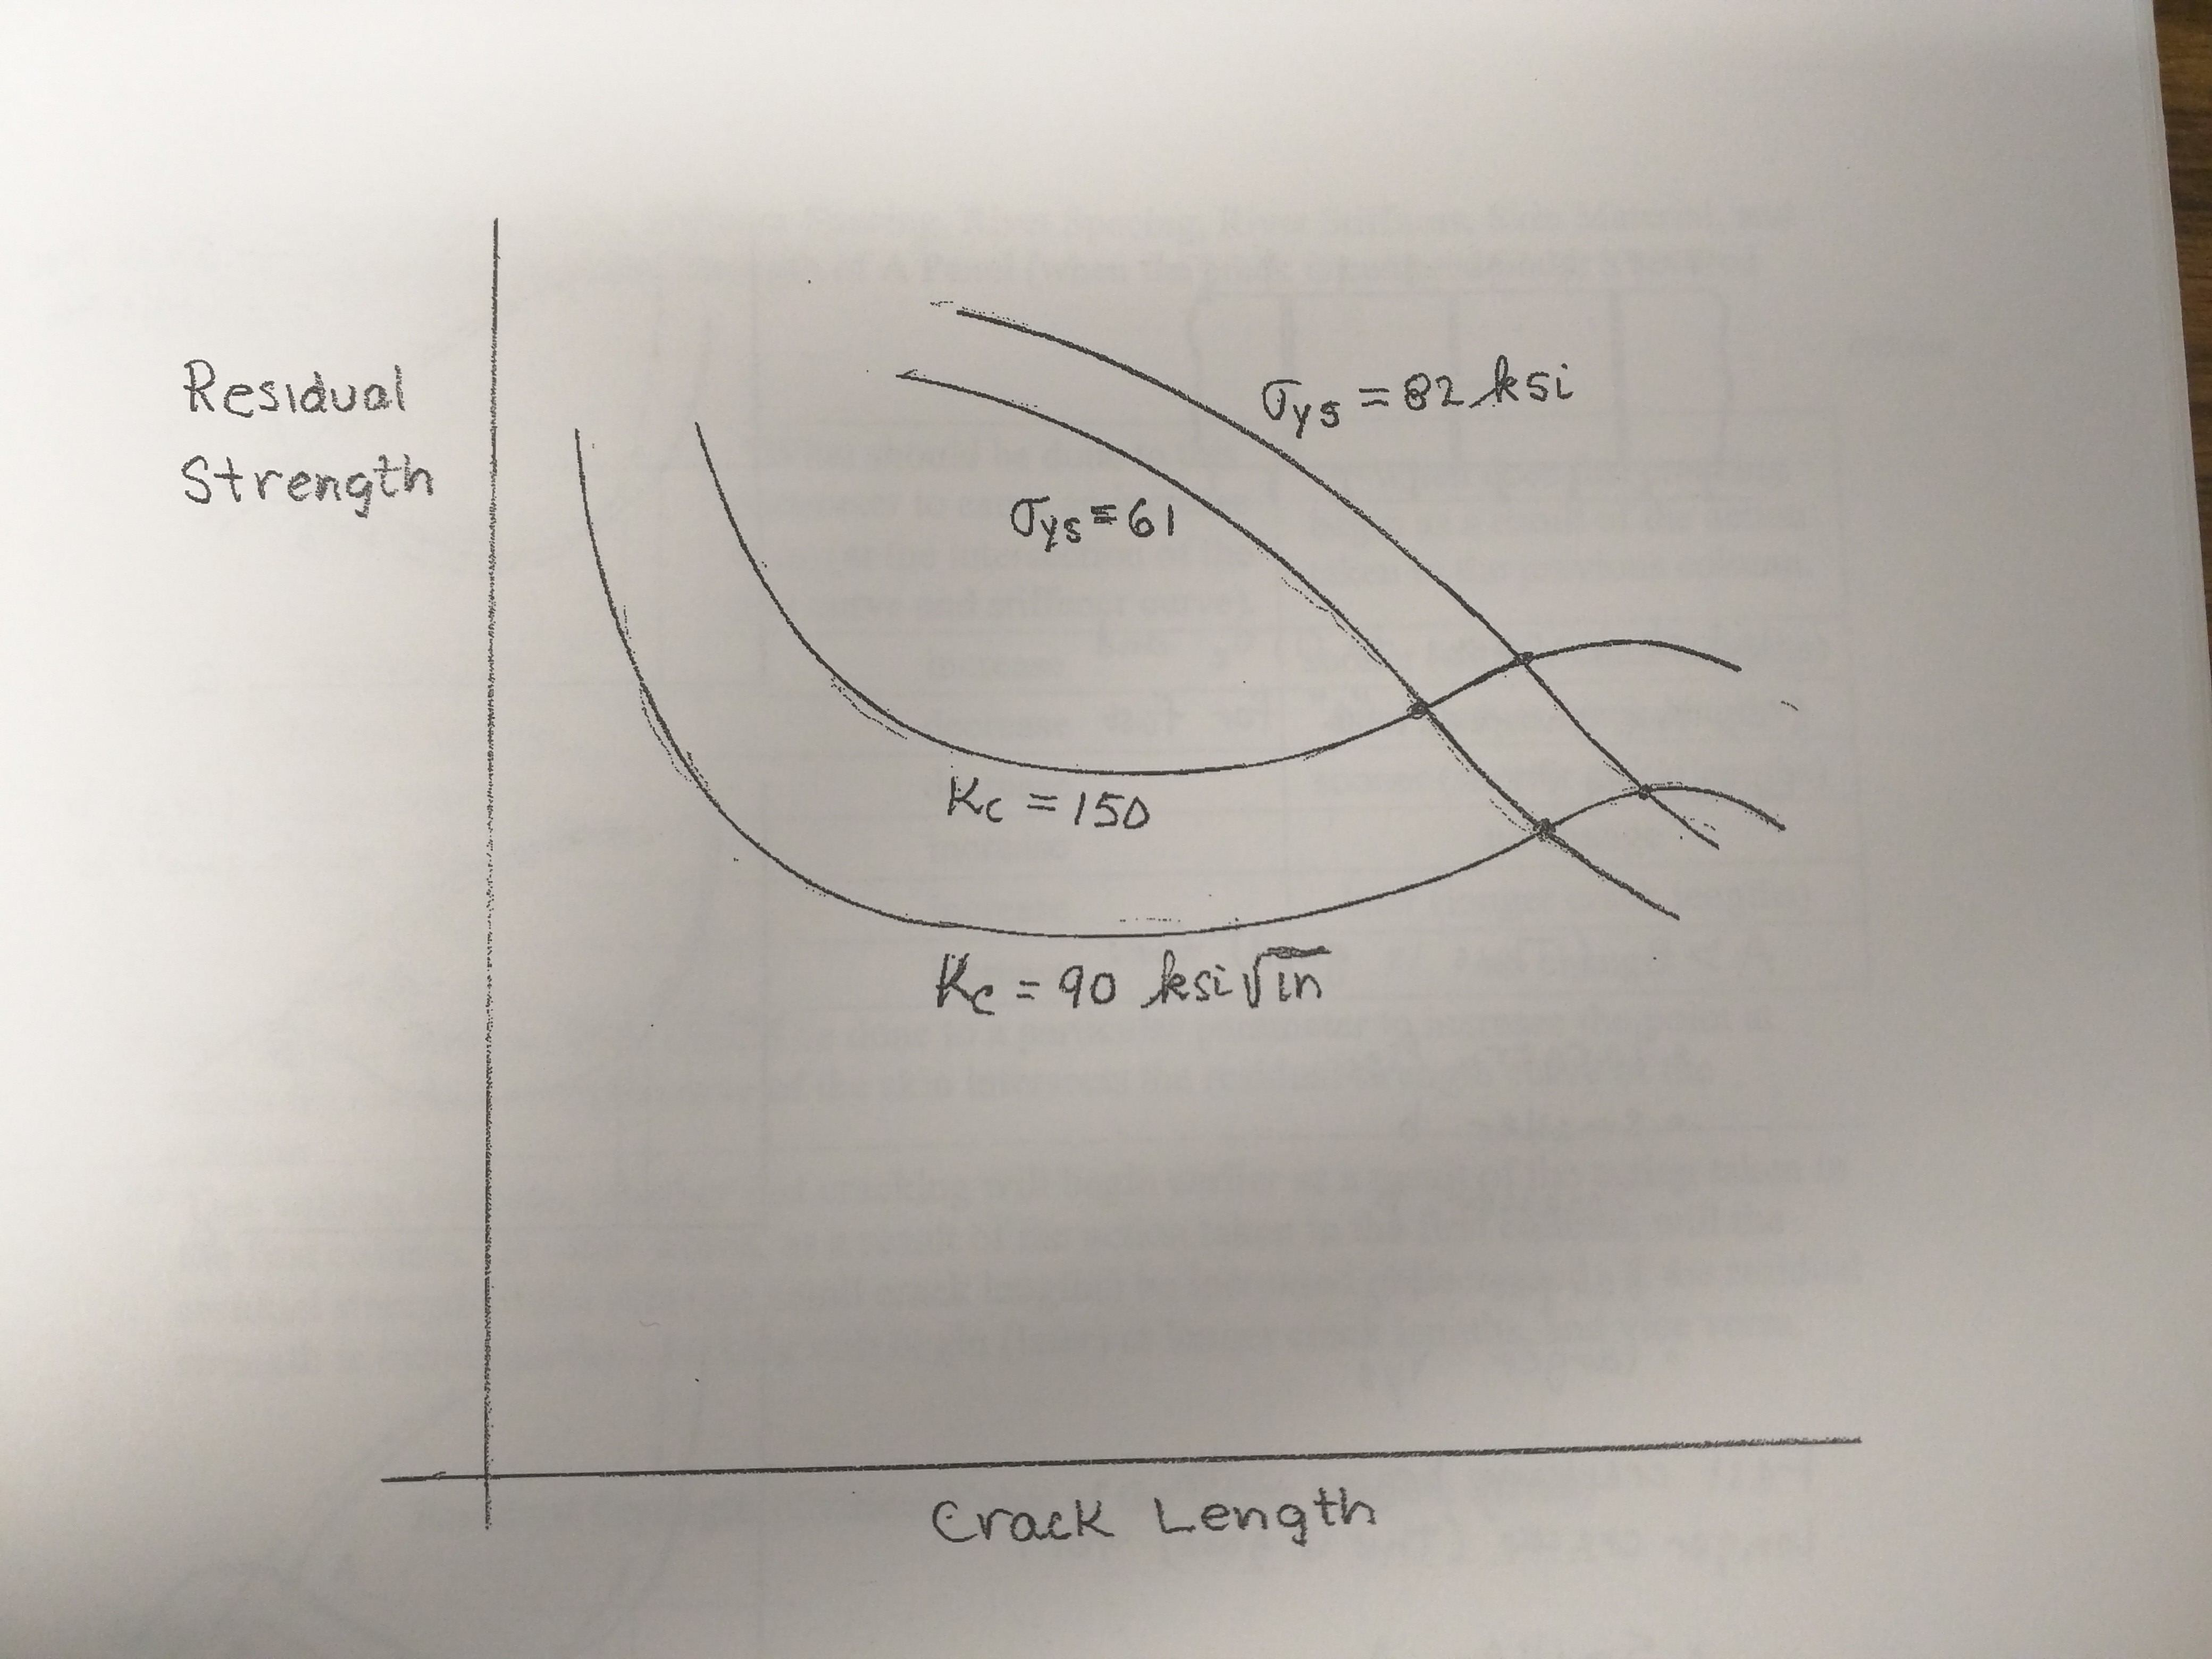
\includegraphics[width=0.7\linewidth]{strength_increase}
\label{fig:strength_increase}
\end{figure}
\end{frame}

\begin{frame}{example}
	\begin{itemize}
		\item If we consider the case from Swift's data most similar to our previous example:
		\begin{align*}
		P &= 1.0 \text{ in}\\
		A_{st} &= 0.2538 \text{ in}^2\\
		b &= 10.0 \text{ in}\\
		\end{align*}
		\item So we use the tables for Case 10
	\end{itemize}
\end{frame}

\section{crack stoppers}

\begin{frame}{crack stopper}
\begin{figure}
\centering
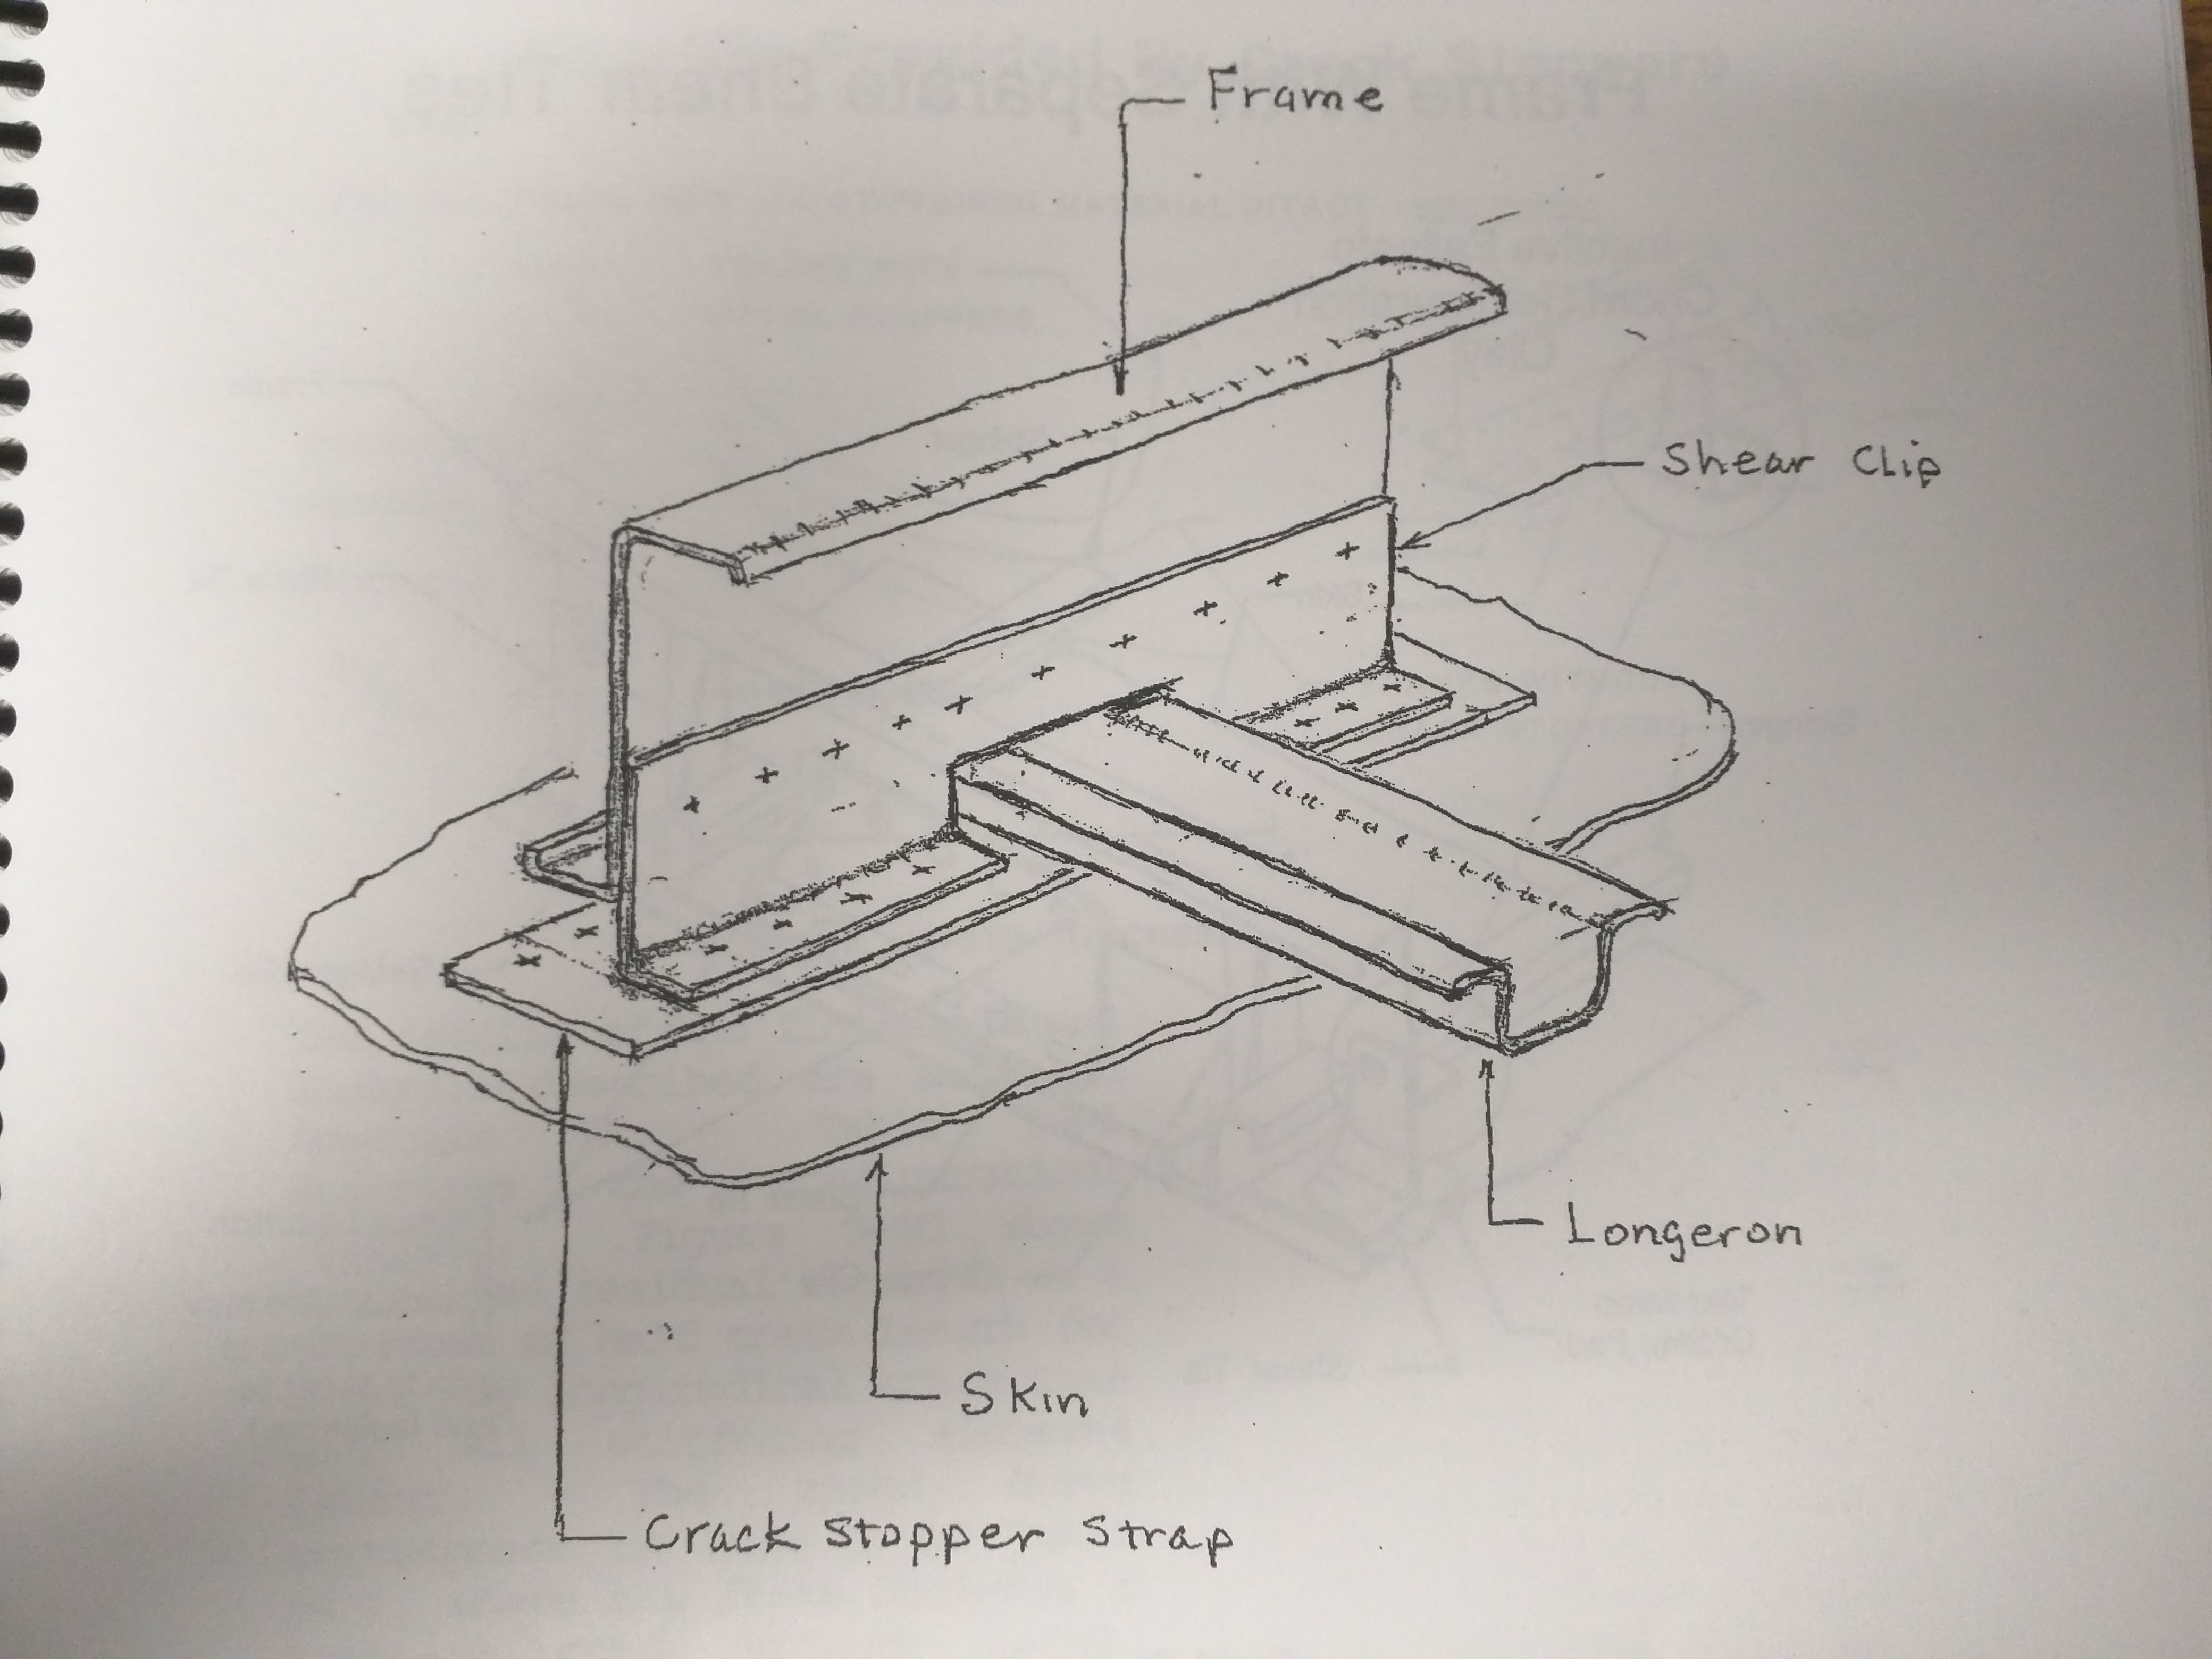
\includegraphics[width=0.7\linewidth]{crack_stoppers}
\label{fig:crack_stoppers}
\end{figure}
\end{frame}

\begin{frame}{optimal crack stopper}
	\begin{itemize}[<+->]
		\item Swift found that the ideal crack stopper has a cross-sectional area approximately equal to 1/4 the stiffener area
		\item The ideal material was titanium (as opposed to steel or aluminum).
		\item Aluminum did not transfer enough load to the stiffeners, steel transferred too much
	\end{itemize}
\end{frame}

\begin{frame}{example}
	\begin{itemize}
		\item Compare cases 1, 3, and 5 
	\end{itemize}
\end{frame}

\section{multiple site damage}

\begin{frame}{multiple site damage}
	\begin{itemize}[<+->]
		\item Often damage can accumulate among multiple sources
		\item This is very common when there are a series of holes, each can develop cracks with a potential to link up
		\item "link up" occurs when the plastic zones between two adjacent cracks touch
	\end{itemize}
\end{frame}

%TODO redo figure
\begin{frame}{linkup}
\begin{figure}
\centering
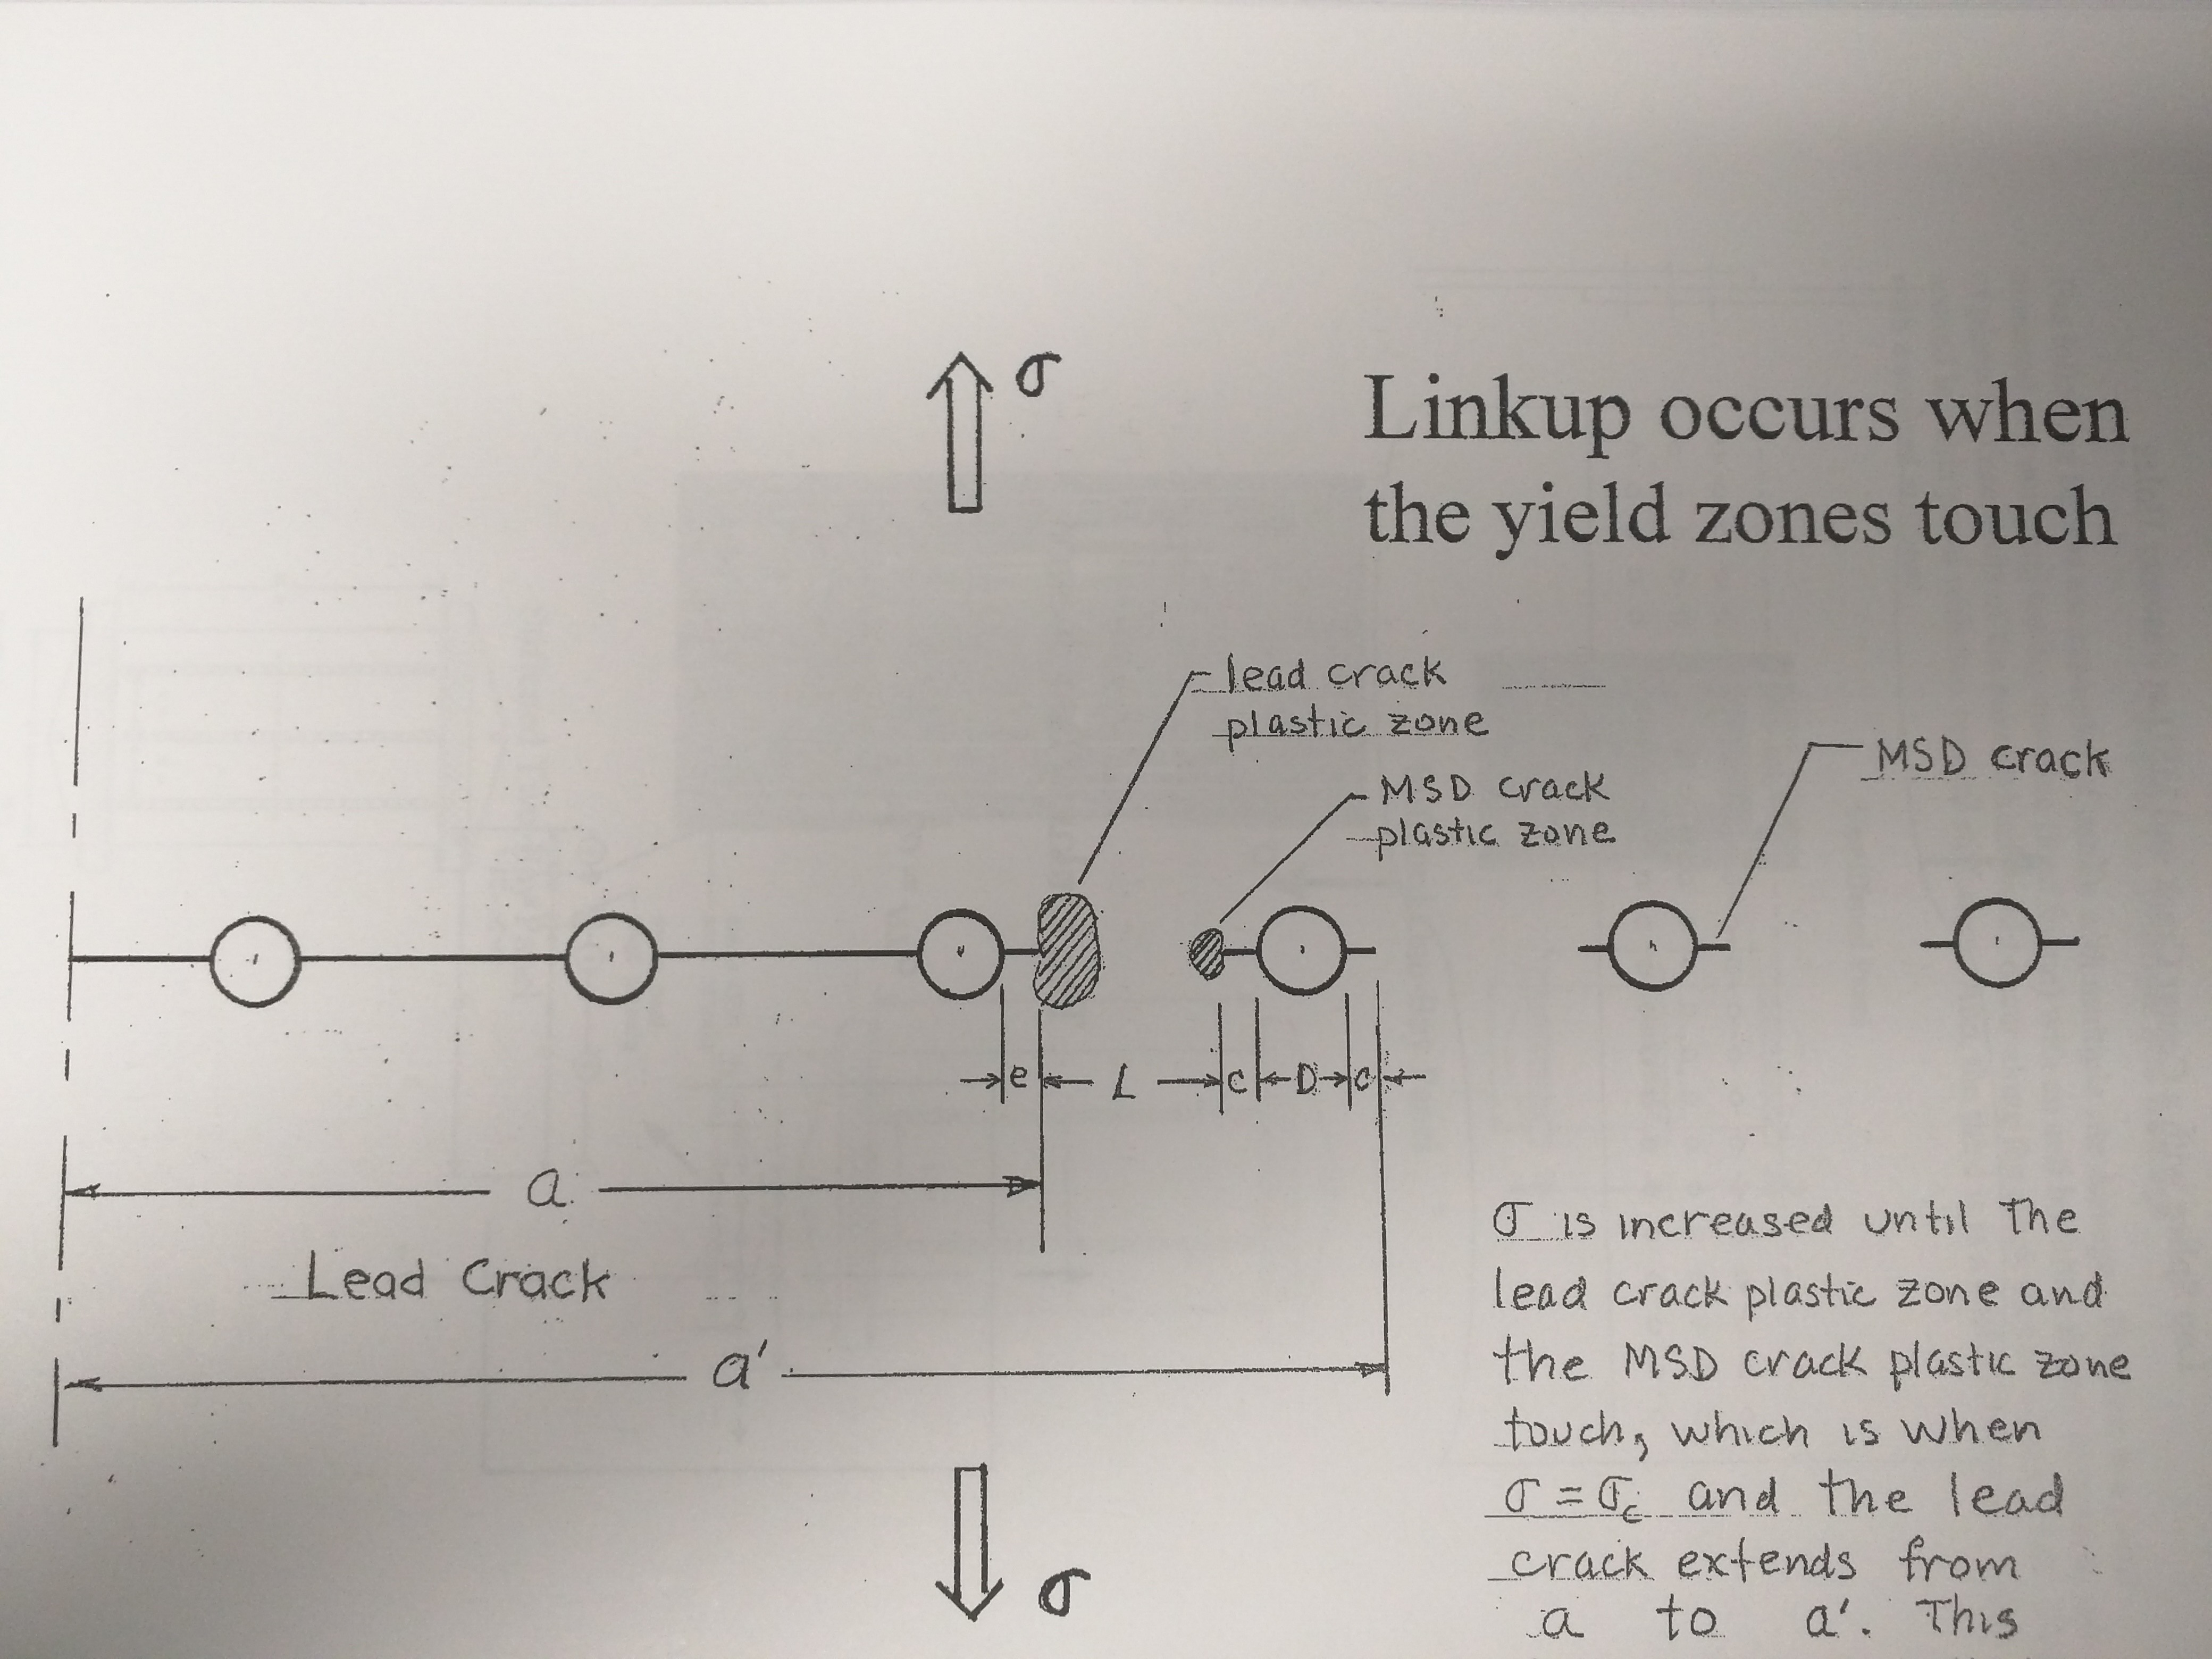
\includegraphics[width=0.7\linewidth]{msd}
\label{fig:msd}
\end{figure}
\end{frame}

%TODO redo figure

\begin{frame}{linkup equation}
	\begin{itemize}[<+->]
		\item We know that
		\begin{equation}
		R_p = \frac{1}{2\pi}\left(\frac{K_{Ia}}{\sigma_{YS}}\right)^2
		\end{equation}
		\begin{equation}
		r_p = \frac{1}{2\pi}\left(\frac{K_{Il}}{\sigma_{YS}}\right)^2
		\end{equation}
		\item Where we define the stress intensity factors at a and L as
		\begin{equation}
		K_{Ia} = \sigma \sqrt{\pi a} \beta_a
		\end{equation}
		\begin{equation}
		K_{Il} = \sigma \sqrt{\pi l} \beta_l
		\end{equation}
	\end{itemize}
\end{frame}

\begin{frame}{linkup equation}
	\begin{itemize}[<+->]
		\item Since fast cracking occurs when $R_p + r_p = L$, we solve for the condition where $R_p + r_p < L$
		\begin{subequations}
		\begin{align}
		\frac{1}{2\pi}\left(\frac{K_{Ia}}{\sigma_{YS}}\right)^2 + \frac{1}{2\pi}\left(\frac{K_{Il}}{\sigma_{YS}}\right)^2 &< L\\
		\frac{1}{2\pi\sigma_{YS}^2} \left[K_{Ia}^2 + K_{Il}^2\right] &< L \\
		\frac{1}{2\pi\sigma_{YS}^2} \left[\sigma^2 \pi a \beta_a^2 + \sigma^2 \pi l \beta_l^2\right] &< L \\
		\frac{\sigma^2}{2\sigma_{YS}^2} \left[a \beta_a^2 + l \beta_l^2\right] &< L \\
		\frac{\sigma_c^2}{2\sigma_{YS}^2} \left[a \beta_a^2 + l \beta_l^2\right] &= L \\
		\sigma_c &= \sigma_{YS}\sqrt{\frac{2L}{a \beta_a^2 + l \beta_l^2}}
		\end{align}
		\end{subequations}
	\end{itemize}
\end{frame}
\end{document}
